\section*{Dati e risultati}

\subsubsection*{Cuore}

Per una migliore comprensione di quello che andreamo a realizzare e studire, in questo primo paragrafo vogliamo dare qualche nozione di base sulla struttura di un cuore umano e del suo funzionamento.

\begin{wrapfloat}{figure}{I}{0pt}
	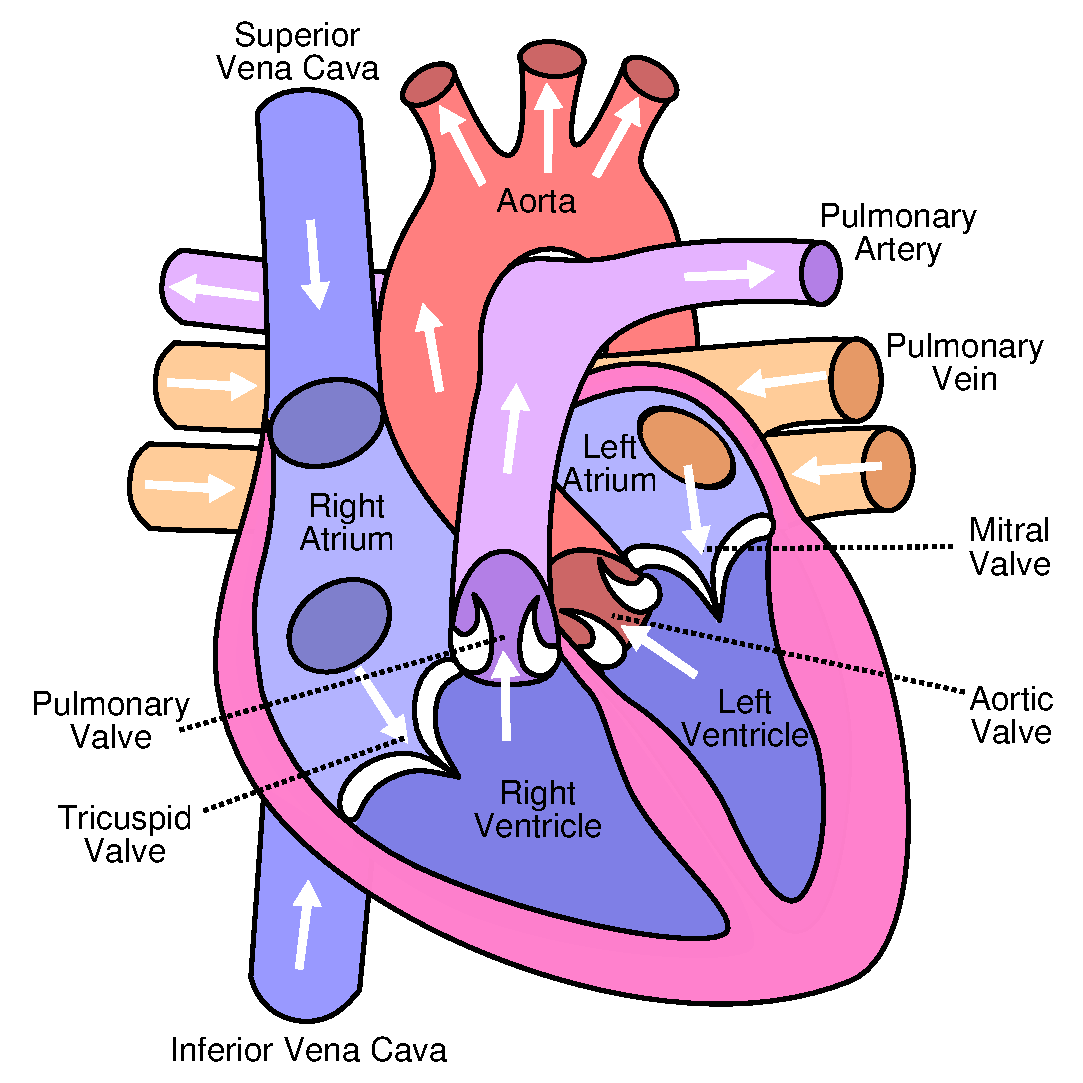
\includegraphics[width=0.5\textwidth]{figure/heart.pdf}
	\caption{Rappresentazone di un cuore umano, con in evidanza le parti più importanti ai fini della nostra trattazione.}
	\label{fig:heart}
\end{wrapfloat}

Il cuore si divide in due cavità, la sinistra dove circola sangue arterioso ricco di ossigeno e la destra dove circola sangue venoso desaturato. Ognuna di queste cavità comprende una parte superiore, atri a pareti sottili, e una parte inferiore, ventricoli a pareti più spesse. Tutto questo è visibile in Figura \ref{fig:heart}.
Il cuore come tutti i muscoli è capace di contrarsi sfruttando l'energia prodotta dall' ossidazione di sostanze energetiche (come acidi grassi, carboidrati) in presenza di ossigeno. 
Il controllo nervoso sul cuore può modulare la frequenza di contrazione aumentandola o diminuendola. La contrazione è generata in maniera spontanea dal miocardio (muscolo cardiaco).
Esiste una parte del miocardio dedicata alla sola generazione e conduzione degli impulsi elettrici attraverso il muscolo cardiaco: il cosiddetto miocardio specifico. Si tratta di un sistema che permette la contrazione di tutte le parti dei ventricoli in maniera pressoché simultanea.
Quindi questo stimolo elettrico che come conseguenza porta alla contrazione della membrana cardiaca in elettronica lo si può approssimare ad un oscillatore che una volta innescato da un impulso inizia ad emettere a sua volta un’onda quadra.

\subsubsection*{Elettrocardiogramma}

L'elettrocardiogramma (ECG) è la riproduzione grafica dell'attività elettrica del cuore durante il suo funzionamento, registrata dalla superficie del corpo.
Il principio che permette la misurazione dell'attività elettrica del cuore si basa sulla generazione di una differenza di potenziale con l'insorgere degli impulsi eletrici nel miocardio. Questa diffrenza di potenziale può essere registrata grazie a degli elettrodi posti sulla superficie corporea. Si osservi che questi impulsi elettrici possono essere letti poichè il corpo umano è un buon conduttore a causa dei liquidi interstiziali presenti in tutto l'organismo.

\subsubsection*{Elettrodo}

Un elettrodo è un conduttore di prima specie (per esempio metallo o grafite) usato per stabilire un contatto elettrico con una parte non metallica di circuito (nel nostro caso la pelle). Grazie a questo componente siamo in grado di misurare la differenza di potenziale dell'impulso emesso dal miocardio e, con il circuito che andreamo a realizzare, potremo visualizzare sull'osciloscopio le varie fasi della contrazione cardiaca.

\subsubsection*{Considerazioni preliminari}

In media sulla superficie corporea la differenza di potenziale del segnale ECG appartiene ad un range compreso tra \SI{-1}{\milli\volt} e \SI{+1}{\milli\volt} (con picchi massimi di circa \SI{4}{\milli\volt}) e frequenza $\nu\ped{cardiaca}$ di circa \SI{1.25}{\hertz}. Gli elettrodi, che permettono il collegamento tra la strumentazione e la superficie corporea amplificano il segnale corporeo di circa 700 volte. Infatti creano differenze di potenziale dell'ordine di \SI{700}{\milli\volt}.

Inoltre la disposizione degli elettrodi sulla superficie corporea è molto varia a seconda del grado di accuratezza che si vuole avere e anche in base a cosa si vuole osservare con esattezza del battito cardiaco. Dal momento che a noi interessa rilevare semplicemente la forma tipica dell'impulso cardiaco, curva periodica detta cardioide, ci accontentiamo di una disposizione semplice ma efficace degli elettrodi. Un elettrodo viene posiszionato sul polso sinistro del paziente, uno su quello destro e l'ultimo sulla caviglia sinistra.

Quindi, tenendo presente quanto detto, possimo intuire che nell'efettuare la misura, ci possono essere molte sorgenti di rumore che porterebbero ad un alterazione della misura. Ad esempio:

\begin{itemize} \itemsep0pt \parskip0pt \parsep0pt
	\item{Movimenti volontari e non del corpo del paziente;}
	\item{Movimenti casuali degli elettrodi o dei cavi di connessione che possono disturbare il segnale;}
	\item{Effetti capacitivi e di induzione sui cavi di collegamento e sul circuito;}
	\item{Effetti capacitivi e di induzione sul paziente;}
\end{itemize}

\subsubsection*{Realizzazione ECG}

Al fine di realizzare un circuito che ci permettesse di visualizzare correttamente il segnale elettrico emesso dal miocardio ed eliminare la maggior parte del rumore possibile dal nostro segnale in ingresso $V\ped{heart}$ abbiamo realizzato il circuito illustrato in Figura \ref{fig:ecg}.
Nella sua realizzazione abbiamo tenuto conto dei seguenti parametri: era necessario amplificare il segnale in ingresso $V\ped{heart}$ ed elaborarlo ai fini di pterne dare una rappresentazione chiara sull'oscilloscopio. Occorre separare il segnale utile dai disturbi e attenuarne il rumore. Quindi si deve filtrare.

Detto questo andiamo pertanto ad esaminare il nostro circuito per capire esattamente quale sia lo scopo ed il funzionamento di ciascun elemento.

Il segnale dei due elettrodi $V\ped{dx}$ (polso destro) e $V\ped{sx}$ (polso sinistro) vengono portati ai due ingressi dell'amplificatore operazionale AD622 (U1). I due segnali, prima di entrare ai due ingressi vengono filtrati grazie ai filtri passa basso costituiti dalle resistenze $R_f$ e dai condensatori $C_c$. Inoltre con la presenza del condensatore $C_m$ i due ingressi sono messi in comunicazione ed è quindi possibile eliminare le parti di segnale con frequenze molto elevate. Infatti se indichiamo con $\nu\ped{com0}$ la frequenza di taglio in modo comune e $\nu\ped{diff0}$ quella in modo differenziale abbiamo che:

\begin{equation}
	\nu\ped{com0}\,=\,\frac{1}{2\,\pi\,R\,C_c}\,=\,\SI{4}{\kilo\hertz} \qquad \text{e} \qquad \nu\ped{diff0}\,=\,\frac{1}{2\,\pi\,(2C_m\,+\,C_c)}\,=\,\SI{194}{\hertz}
\end{equation}

In questo modo per il segnale in modo comune ($V^+=V^-$), ottenuto grazie al collegamento dei due ingressi mediante il condensatore $C_m$, viene eliminata la parte di segnale con frequenze superiori alla frequenza di taglio $\nu\ped{com0}$, mentre per il segnale in modo differenziale, quando $V^+ \neq V^-$, vengono eliminate le componenti con frequenza superiore a $\nu\ped{diff0}$. Grazie a questo, visto che $\nu\ped{cardiaca}\,\simeq\,\SI{1.25}{\hertz}$, abbiamo tagliato tutte le componenti di $V\ped{heart}$ con frequenze superiori a quella interessata. Questo ci permette di ridurre, in parte, gli effetti di rumore esterni.

A questo il segnale entra nell'amplificatore differenziale. Le sue funzioni principali sono quelle di eliminare l'effetto del rumore in modo comune presente ad entrambi gli ingressi quindi di fornire in uscita un segnale che corrisponde solo alla differenza tra i suoi due ingressi ($V^+-V^-$). Inoltre vogliamo che $V\ped{heart}$ venga amplificato dal momento che è dellordine dei milli volt.
Dal momentoche abbiamo scelto come valore di resistenze $R_g\,=\,\SI{220}{\ohm}$ il guadagno $G$ dell'amplificatore può essere ricavato con la seguente relazione:

\begin{equation}
	G\,=\,\frac{\SI{50.5}{\kilo\ohm}}{2\,R_g} + 1 \,\simeq\,116 
\end{equation}

quindi il segnale in ingresso viene amplificato di circa 116 volte.

Successivamente il segnale in uscita dall'amplificatore operazionale, $V\ped{out1}$ viene filtrato grazie al filtro passa alto formato dalla resistenza $R_1$ e dalla capacità $C_1$. Questo filtro ha una frequenza di taglio di circa \SI{3}{\hertz}, quindi molto bassa. Grazie a questo si riescono ad eliminare le componenti continue del segnale in uscita con frequenza pari o inferiore ai \SI{3}{\hertz}.
A questo punto il segnale passa per l'amplificatore operazionale OP07 in configurazione di ``emitter follower'' (U2) che presenta pertanto un'elevanta imedenza di ingresso.

Successivamente, il segnale in uscita da questo secondo amplificatore, $V\ped{out2}$, passa per un ulteriore amplificatore operazionale OP07 (U3). Questo amplificatore è in configurazione invertete con guadagno $G\,=\,-10$. La presenza del condensatore $C_2$ serve per eliminare ulteriormente le componenti del segnale in ingresso ad alta frequenza. Infatti queste non vengono amplificate.

Nel circuito è presente un ulteriore amplificatore operazionale OP07 in configurazione ``emitter follower'' (U4) non invertente. Questo stadio serve per polarizzare ad una tensione pari al modo comune la calza del cavo coassiale che connette gli elettrodi all'amplificatore AD622. In questo modo riduco l’effetto delle capacità parassite e aumento la reiezione di modo comune, quindi l'amplificazione del segnale differenziale risulta più grande di quella del segnale in modo comune. Questo serve per:

\begin{itemize}\itemsep0pt \parskip0pt \parsep0pt
	\item{Il cavo che porta il segnale sente una bassa differenza di potenziale tra il conduttore e l'isolante e quindi limito l'atteuazione del segnale;}
	\item{Entrambe le calze sentono lo stesso potenziale. In questo modo non è influente la loro posizione sul banco di laboatorio;}
\end{itemize}

Infine dobbiamo analizzare il blocco U5 costituito da un amplificatore di isolamento, ISO124. Questo stadio è di fondamentale importanza dal momento che isola galvanicamente le due parti del ``circuito''.
Ovvero da una parte abbiamo l'alimentazione del circuito +VS1\,=\,\SI{+9}{\volt} e -VS2\,=\,\SI{-9}{\volt} fornita dalla serie delle due batterie. Questa differenza di potnziale è riferita a quello che abbiamo indicato come GND1. Mentre l'alimentazione del segnale in uscita, che poi deve essere trasmesso all'oscilloscopio, è alimentata con $\pm VS2$  che fanno riferimento a GND2. Le due masse sono chiaramente differenti e separate in modo tale da non creare giri di massa che possano mettere in pericolo la vita paziente.
Quindi le due parti del circuito sono isolate, ma il segnale in uscita dal blocco U3 quindi entrante nell'ISO124 e uscente dallo stesso sono uguali. Questo segnale è quindi il risultato finale di tutti gli accorgimenti illustrati fino ad ora e rappresenta pertanto il nostro segnale ECG.

Quindi nelle Figure \ref{fig:ecg_normale} e \ref{fig:ecg_corsa} riportiamo i risultati ottenuti grazie al circuito realizzato in Figura \ref{fig:ecg}.

\begin{SCfigure*}[][h]
    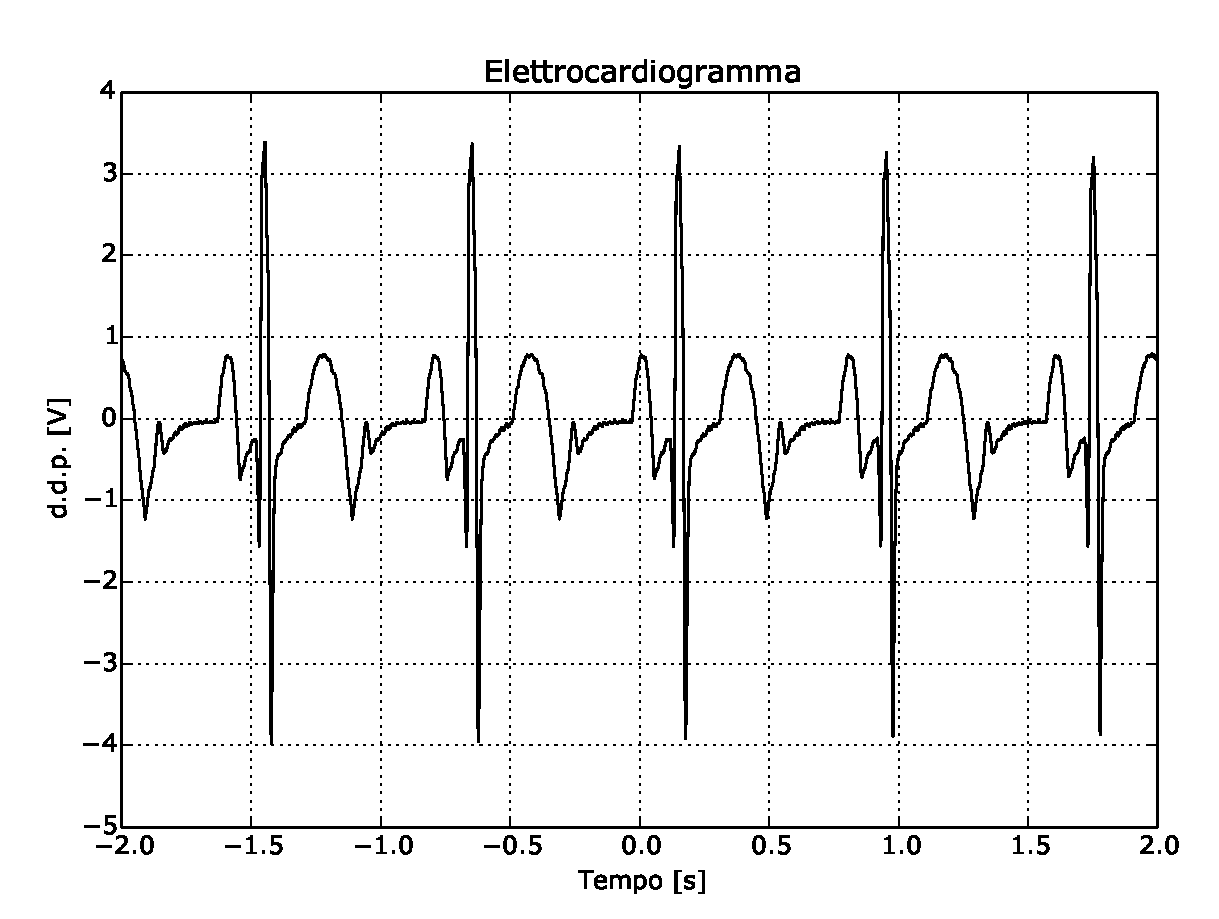
\includegraphics[height=0.4\textheight]{figure/ecg.pdf}
    \caption{Elettrocardiogramma acuisito durante la sessione di laboratorio. Il battito cardiaco é di 75 battiti/minuto. Infatti possiamo notare che l'intervallo temporale tra un picco ed un altro è di circa \SI{800}{\milli\second} con un errore di \SI{2}{\milli\second}. Sono inoltre visibili altri picchi secondari, dovuti a varie fasi dell'attivitá cardiaca.}
    \label{fig:ecg_normale}
\end{SCfigure*}

\begin{SCfigure*}[][h]
    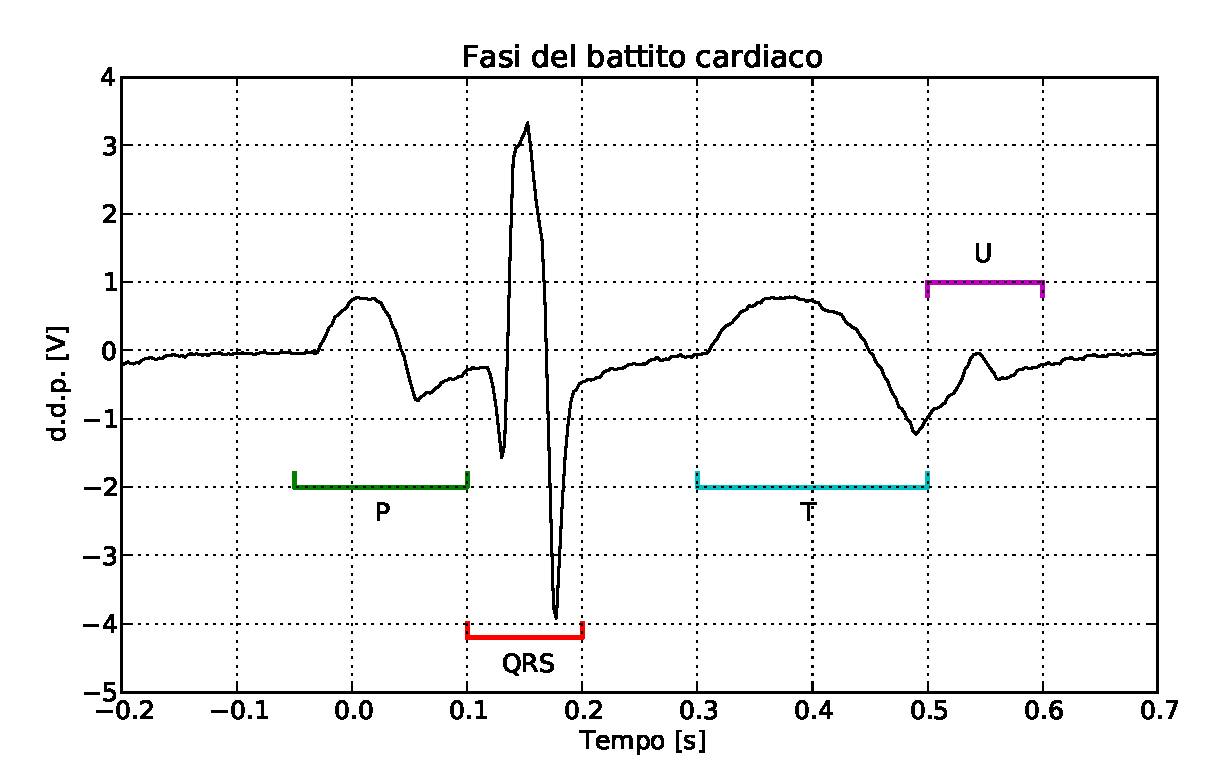
\includegraphics[height=0.35\textheight]{figure/ecg_fasi.pdf}
    \caption{Questa è un immagine illustrativa di un ECG ideale nel quale è possibile identificare le quattro fasi principali dell'attività cardiaca. Fase P, depolarizzazione atrii, fase QRS depolarizzazione ventricoli e polarizzazione atrii, fase T, polarizzazione atrii e infine fase U, polarizzazione muscoli papillari.}
    \label{fig:ecg_ideale}
\end{SCfigure*}

A questo puto è doverose dare una minima nozione del significato dei vari picci principali e secondari che sono presenti negli ECG eseguiti. A tal fine in Figura \ref{fig:ecg_ideale} è riportato l'andamento di un elettrocardiogramma ideale.
Come è intuibile dai risultati ottenuti il normale tracciato ECG (Figura \ref{fig:ecg_ideale}) presenta un aspetto caratteristico che varia soltanto in presenza di problemi. Il tracciato è caratterizzato da diversi tratti denominati onde, positive e negative, che si ripetono ad ogni ciclo cardiaco.
Le differenze principali tra queste onde sono elencate di seguito:

\begin{itemize} \itemsep0pt \parskip0pt \parsep0pt
	\item{Onde P: è la prima onda che si genera nel ciclo. Corrisponde alla depolarizzazione degli atri ovvero il sangue viene pompato dagli atrii ai ventricoli;}
	\item{Complesso QRS: si tratta di un insieme di tre onde che si susseguono l'una all'altra, e corrisponde alla depolarizzazione dei ventricoli. Ovvero si tratta del momento in cui il sangue viene pompato dai ventricoli verso la Aorta o l'Arteria polmonare, quindi quando il sangue viene immesso in circolo. Durante questa fase avviene anche la polarizzazione degli atrii, ovvero questi si riempiono di sangue che poi dovrà essere pompato nei ventricoli;}
	\item{Onda T:rappresenta la polarizzazione dei ventricoli. Quindi il momento in cui i ventricoli si riempiono di sangue prelevandolo dagli atrii. Non sempre è identificabile, perché può anche essere di valore molto piccolo;}
	\item{Onda U: è un'onda che non sempre è possibile apprezzare in un tracciato, dovuta alla polarizzazione dei muscoli papillari;}
\end{itemize}

\begin{SCfigure*}[][h]
    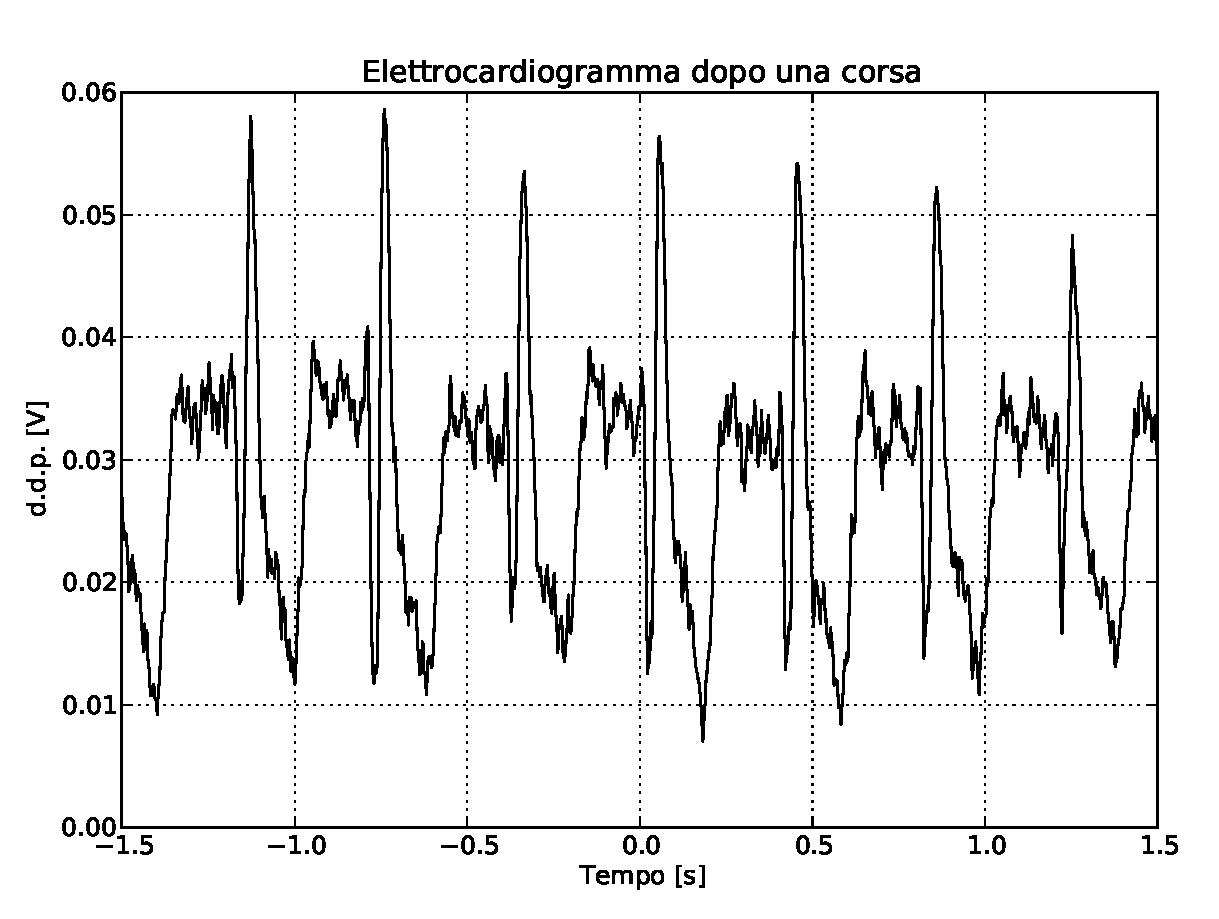
\includegraphics[height=0.4\textheight]{figure/ecg_corsa.pdf}
    \caption{Elettrocardiogramma dello stesso soggetto dell'ECG in Figura \ref{fig:ecg_normale} soltanto che in questo caso il paziente é uscito dal laboratorio e ha percorso qualche centinaio di metri di corsa prima della misura. Di conseguenza, il battito é salito a circa 150 battiti/minuto dal momento che la distanza tra due picci è di circa \SI{400}{\milli\second} con una precisione di qualche millisecondo. SI può osservare come questo ECG sia poco piú rumoroso del precedente.}
    \label{fig:ecg_corsa}
\end{SCfigure*}

%\begin{wrapfloat}{figure}{O}{0pt}
%        \def\svgwidth{0.4\textwidth}
%        \subimport{figure/}{raddrizzatore.pdf_tex}
%        \caption{Raddrizzatore di precisione a semionda. Alimentato, inizialmente con una $V\ped{in}\,=\,\SI{1.02}{\volt}$ di frequenza $\nu\,=\,\SI{50}{\hertz}$.}
%        \label{fig:radd}
%\end{wrapfloat}

%\begin{SCfigure}[][p]
%        \centering
%        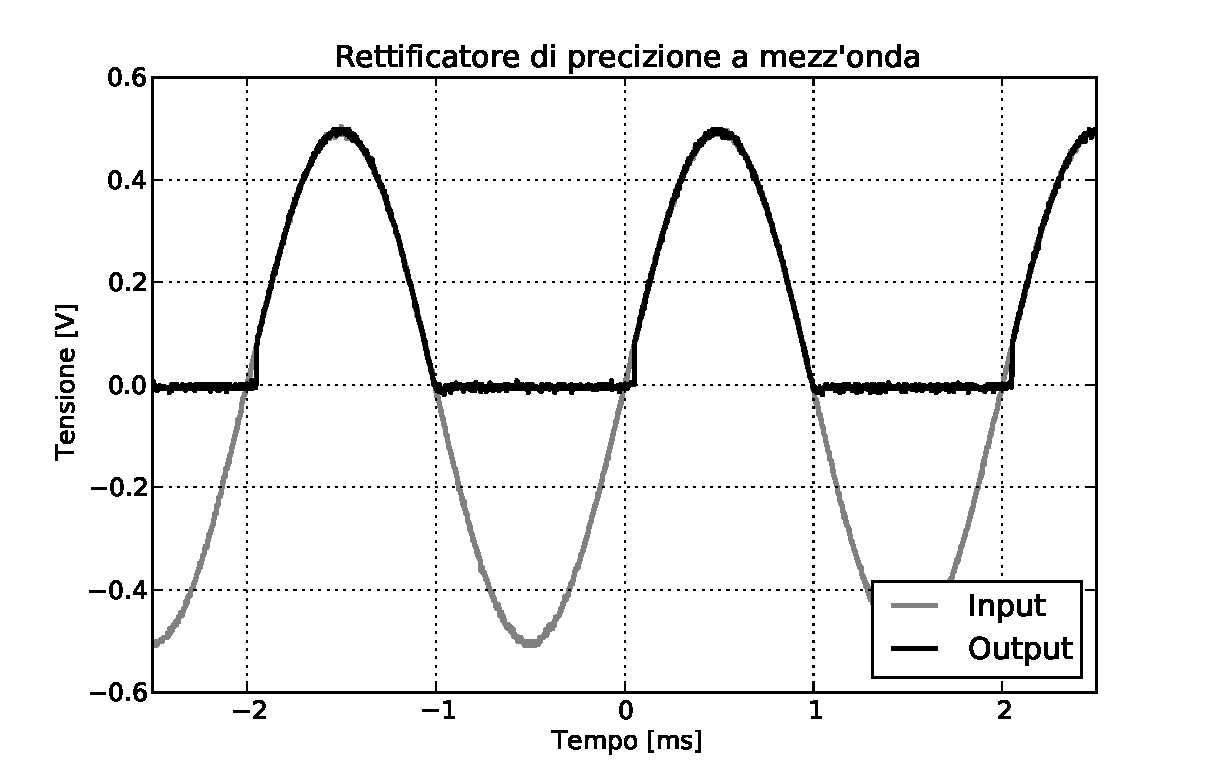
\includegraphics[width=0.7\textwidth]{figure/rett.pdf}
%        \caption{Questo grafico illustra l'andamento di $V\ped{out}$, linea nera, in funzione di $V\ped{in}$, linea grigia. Si nota chiaramente, come da previsioni, che la parte negativa del segnale in ingresso impediscse al diodo di condurre, pertanto la tensione di output risulta nulla. Inoltre, come si può osservare, il fronte di salita di $V\ped{out}$ presenta un leggero ritardo rispetto al segnale in ingresso $V\ped{in}$. Questo ritardo è stato stimato essere approssimativamente di circa $(152\pm10)\SI{}{\micro\second}$.}
%        \label{fig:radd_plot1}
%\end{SCfigure}
